\newcommand\textschwa{\rotatebox{180}{\parbox[t][0.5em][c]{0.5em}{e}}}

\PrerenderUnicode{ş}
\PrerenderUnicode{ı}
\PrerenderUnicode{ğ}
\PrerenderUnicode{à}

\newcommand\turcodocslice[3]{
  \begin{center}
    \begin{tabular}{c}
      \includegraphics{parole/#1.png}\\[1cm]
      \RL{#2}\\[1cm]
      #3\\
    \end{tabular}
  \end{center}
}

\newcommand\frameturcodocslice[5]{
  \myframe{#1}{frame:#2}{
    \setfarsi
    \novocalize
    \turcodocslice{#3}{#4}{#5}
  }
}

\selectlanguage{italian}

\mode
<presentation>
{
  \usetheme{TURCO}
  \setbeamercovered{transparent}
}

\mode
<all>

%\mytitle{Documento 1099}{Documento 1099}{Seminari di LLC Turca}

%\mytitle{Una lettera privata}{Notizie linguistiche e storiche sull'ottomano del 1600. Analisi di una lettera di Ca\Ayn{}fer Paşa, ex-beylerbeyi di Cipro, al doge di Venezia}

\mytitle{Notizie sull'ottomano del 1600}{Notizie linguistiche e storiche\\ sull'ottomano del 1600.\\ Analisi di una lettera di Ca\Ayn{}fer Paşa,\\ ex-beylerbeyi di Cipro, al doge di Venezia}{}

\myauthor{Chiara Paci}

\myinstitute{Tesi di laurea in Lingue e culture dell'Eurasia e del Mediterraneo}

%\date{\today}
\date{22 marzo 2010}

\mode
<presentation>

\pgfdeclareimage[height=0.8cm]{plogo}{logo}
\logo{\pgfuseimage{plogo}}
% Delete this, if you do not want the table of contents to pop up at
% the beginning of each subsection:
\AtBeginSection[]{
  \begin{frame}<beamer>
    \frametitle{Indice}
    \tableofcontents[sectionstyle=show/shaded,subsectionstyle=hide/hide/hide]
  \end{frame}
}

\mode
<all>

\begin{document}
\novocalize
\setcnash
\setottoman
\settrans{ottoman}
\setnoquot % per le figure con pgf/tikz: altrimenti non si può usare <->

\openpresentazionenotoc

\mode
<all>


\mysection{Introduzione}

\myframe{Documento}{frame:doc1099}{
\begin{center}
\begin{tabular}{cc}
  \multicolumn{2}{c}{\only<2>{1601}}\\
  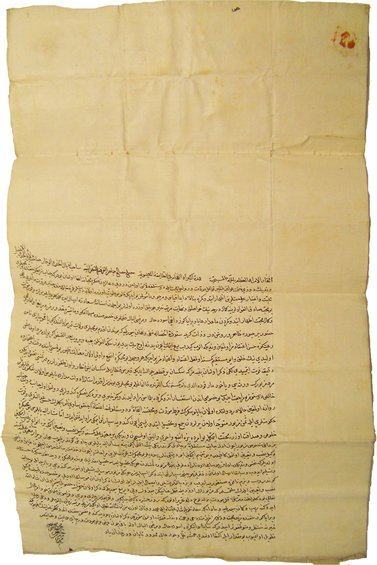
\includegraphics{rdoc1099r-rid.jpg} &
  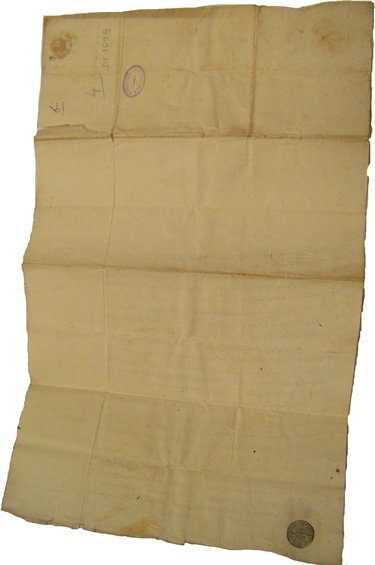
\includegraphics{rdoc1099v-rid.jpg} \\
\end{tabular}
\end{center}
}

\myframe{Regesto}{frame:regesto}{
  \begin{center}
    {\scriptsize
      
      \begin{tabular}{p{2cm}cr}
        &Cose turchi&N$^\text{o}$ 379\\[2mm]
        &Sine data&\\[2mm]
        \multicolumn{3}{c}{
          \parbox{7.5cm}{Lettera in  turco diretta al  
            {\only<3>{\color{evidenzia}\bf}Doge di Venezia}
            da {\only<2>{\color{evidenzia}\bf}Gefer Bassà fu Beglierbei di Cipro} nella quale si lagna
            della    perdita     fatta    di    alcune     balle    di
            Bombace.}}\\
        &Originale e traduzione.&\\
      \end{tabular}
    }

    \parbox[b][6cm][c]{10cm}{\centering
      \only<1>{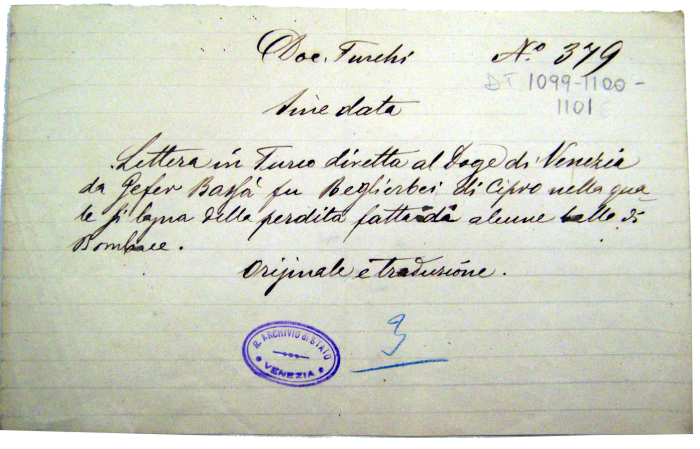
\includegraphics[scale=0.28]{regesto.png}}
      \only<2>{\begin{tabular}[b]{cc}
          \includegraphics[scale=0.18]{documenti/vecellio295.png}&
          \includegraphics[scale=0.3]{ritratti/nadiri-rid.jpg}\\ 
          \resizebox{3cm}{!}{\parbox{8cm}{{\sc Cesare Vecellio}, {\it Habiti antichi et moderni di tutto il mondo}, Venezia, 1598}}
          & \resizebox{3cm}{!}{\parbox{8cm}{{\it  Musicisti di fronte  a Mehmed  III}, Topkapı  Sarayı Müzesi,
              inv.  H889, f.  8, XVII  sec.}} \\
        \end{tabular}}
      \only<3>{\begin{tabular}[b]{lr}
          \includegraphics[scale=0.25]{ritratti/marino_grimani.jpg}&
          \begin{tabular}[b]{r}
            {\tiny Marino Grimani}\\
            {\tiny 1532-1605, doge dal 1595}\\[0.5cm]
            \resizebox{3cm}{!}{\parbox{8cm}{Gabriele Caliari, {\it Il doge Marino Grimani riceve l'ambasciatore persiano}, Venezia, Palazzo Ducale, XVI sec.}}\\
          \end{tabular}\\
        \end{tabular}
      }
    }
    
  \end{center}
}

\myframe{Lingua}{frame:lingua}{
  \begin{tikzpicture}[x=2cm,y=2cm,node distance=1,
      linea/.style={line width=2pt,draw=red},
      lineb/.style={line width=2pt,draw=black},
      linec/.style={line width=2pt,draw=white},
    ]
    \node (docpos) {\includegraphics{img/doc-rid.jpg}};
    \node (poesiapos) at ($(docpos)+(3,1)$) {};
    \node (bazarpos) at ($(docpos)+(3,-1)$) {};
    \only<2->{
      \node (a) at (poesiapos) {\includegraphics[scale=0.5]{img/poesia-rid.jpg}};
    }
    \only<2>{
      \draw[<->,linea] (a) to (docpos);
    }
    \only<3->{
      \node (b) at (bazarpos) {\includegraphics[scale=0.5]{img/bazar-rid.jpg}};
    }
    \only<3> {
      \draw[<->,linea] (b) to (docpos);
      \draw[<->,lineb] (a) to (docpos);
    }
    \only<4>{
      \draw[linea] ($(docpos)+(-1,-1.5)$) rectangle ($(docpos)+(1,1.5)$);
      \draw[->,linea] ($(docpos)+(1,0)$) to ($(docpos)+(3,0)$);
    }
  \end{tikzpicture}
}



\mysection{Il documento}

\myframe{Testo}{frame:testo}{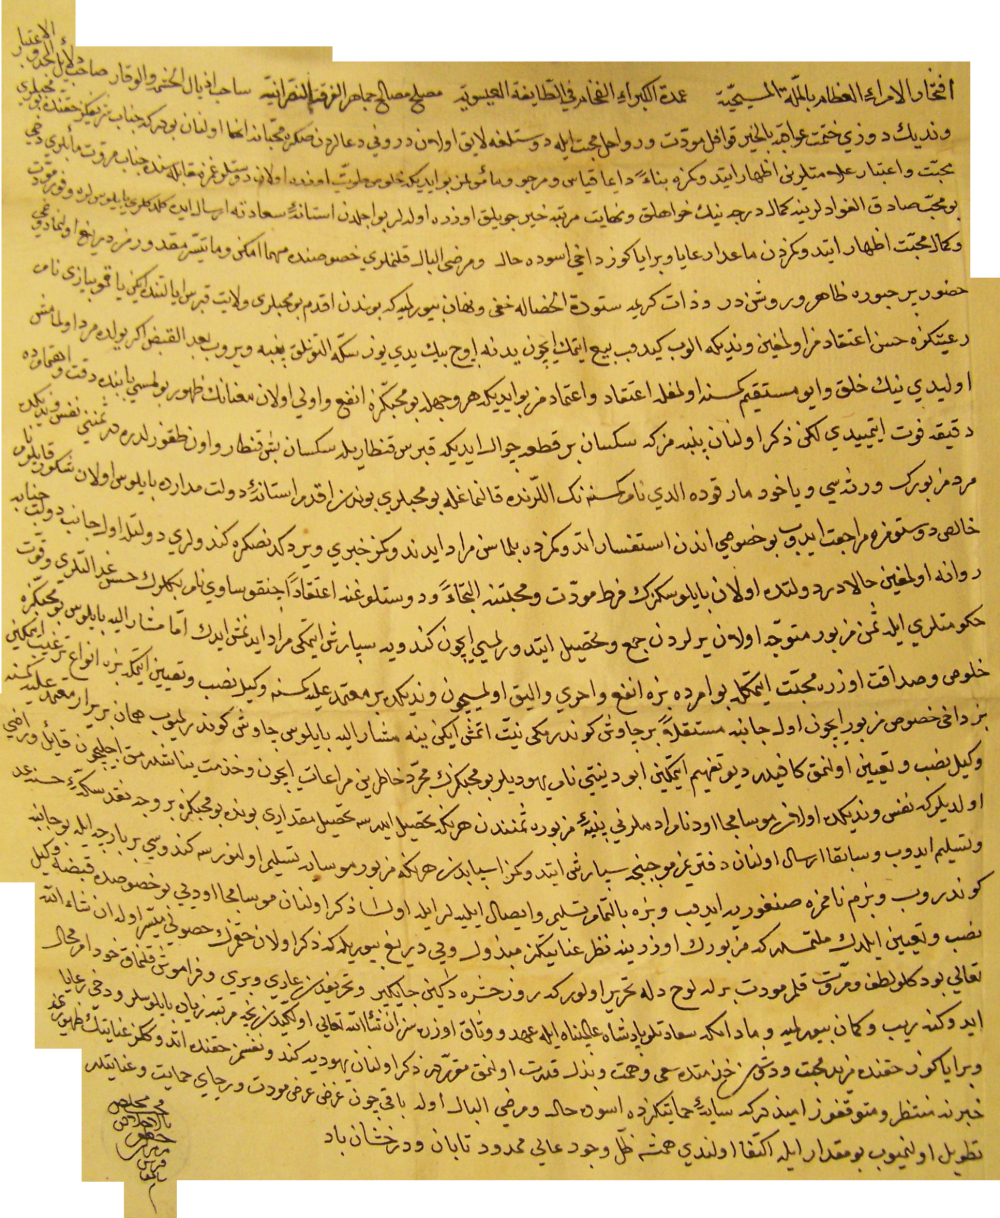
\includegraphics[scale=0.6]{testo.png}}

%% \myframe{Corrispondenti}{frame:corrispondenti}{
%%   \begin{tabular}{cc}
%%    \includegraphics[scale=0.3]{parole/cafertot-rid.jpg}&
%%    \includegraphics{parole/venedik_duzi.png}\\
%%    \spzrlvert[4.5cm]{mu.hibb  mu_halli.s bi-al-a_hlAqyy ^ga`afir  mIrimIrler qubris sAbiqAm} 
%%    & \footnotesize\spzrlvert[3cm]{:vened.Ik d.O^z:I} 
%%    \\
%% \end{tabular}}

\myframe{Cipro}{frame:kibris}{
\setarab
\novocalize
\begin{center}
\begin{tabular}{l@{\hspace{2cm}}r}
  \multicolumn{2}{c}{\includegraphics{parole/kibris_vilayet.png}}\\
  \spzrl{b.U mu.hiblarI wilAyat qubris ayAlatind:H .Jken}{}\\[1cm]
  \multicolumn{2}{c}{
    \parbox[c]{0.58\textwidth}{\centering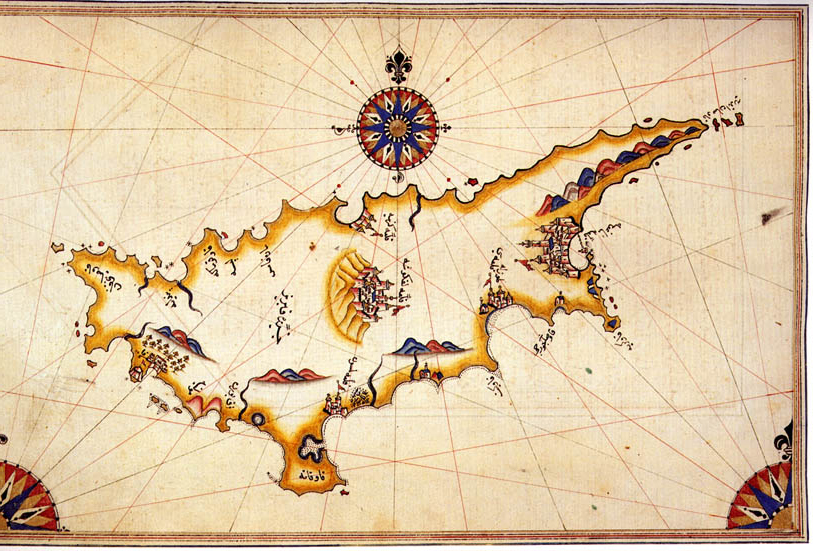
\includegraphics{atlas/Cyprus_by_Piri_Reis.jpg}}
    \parbox[c]{0.35\textwidth}{\tiny {\sc Piri Reis}, {\it Kitab-ı Bahriye}, 1521-25}}\\
\end{tabular}
\end{center}
}

%% \myframe{Giacomo Biasii}{frame:yaqumu}{
%% \setfarsi
%% \novocalize
%% \parbox[c]{0.48\textwidth}{
%%   \begin{tabular}{c}
%%     \includegraphics{parole/yaqum_biazii.png}\\
%%     \spzrl{y^Aqom.O||by^Az.Y nAm}\\
%%     \includegraphics{parole/rayetinize.png}\\
%%     \spzrl{ra`iyati^niz.H}\\
%% \end{tabular}}\hfill\parbox[c]{0.5\textwidth}{\centering
%%   \begin{tabular}{p{0.48\textwidth}}
%%     \includegraphics[scale=0.3]{documenti/vecellio321.png}
%%     \includegraphics[scale=0.3]{ritratti/mercante2.png}\\[0.2cm]
%%     {\tiny {\sc Cesare Vecellio}, {\it Habiti antichi et moderni di tutto il mondo}, Venezia, 1598}\\
%%   \end{tabular}}
%% }

%% \myframe{Cotone}{frame:penbe}{
%%   \setfarsi
%%   \novocalize
%%   \parbox[c]{0.4\textwidth}{\centering\begin{tabular}{c}
%%       \includegraphics{parole/penbe.png}\\[1cm]
%%       \spzrl{penb.H}\\[1cm]
%%   \end{tabular}}
%%   \hfill\parbox[c]{0.55\textwidth}{
%%     \begin{tabular}{c}
%%       \includegraphics[scale=0.6]{documenti/alpino.jpg}\\
%%       {\tiny {\sc Prosper Alpinus}, {\it De Plantis Aegypti Liber}, Venezia 1592}\\
%%   \end{tabular}}
%% }

\presspzrlvert[7cm]{Peso}{kantar}{kantar.png}
              {qubris  qan.tAr.Il.H seks^En  be^s qan.tAr wa .Qn .toq.Uz lodr.H}

%% \myframe{Peso}{frame:kantar}{
%%   \setfarsi
%%   \novocalize
%%   \begin{center}
%%     \begin{tabular}{c}
%%       \includegraphics{parole/kantar.png}\\[0.5cm]
%%       \spzrlvert[7cm]{qubris  qan.tAr.Il.H seks^En  be^s qan.tAr wa .Qn .toq.Uz lodr.H}\\
%%     \end{tabular}
%%   \end{center}
%% }


\myframe{Quantità}{frame:cuval}{
  \setfarsi
  \novocalize
  \parbox[c]{0.5\textwidth}{\centering\begin{tabular}{c}
      \includegraphics{parole/cuval.png}\\[1cm]
      \spzrlvert{seks^En  bir qi.ta`_H  ^cu:vAl}\\[1cm]
  \end{tabular}}
  \hfill\parbox[c]{0.4\textwidth}{
    \begin{tabular}{c}
      \includegraphics[scale=0.3]{documenti/luzerner.png}\\
      {\tiny {\sc Diebold Schillieg}, {\it Luzerner Chronik}, 1517}\\
  \end{tabular}}
}

\myframe{Prezzo}{sikke}{
  \begin{center}
  \begin{tabular}{c}
    \includegraphics{parole/sikke.png}\\[0.2cm]
    \spzrl{:W^c b.I^n yed.I y:Uz  sikk.H  alt.Unluq}\\[0.2cm]
    \includegraphics{monete/sanmatteo.png}\\[0.2cm]
    {\tiny Caravaggio, {\it Vocazione di San Matteo}, 1599-1600}\\
  \end{tabular}
  \end{center}
}

%% \myframe{A Venezia}{frame:venedige}{
%% \setarab
%% \novocalize
%% \begin{center}
%% \begin{tabular}{c}
%%   \includegraphics{parole/venedikte.png}\\[0.2cm]
%%   \spzrl{:vened.Ik.H  ^Al.Ub g.Id:Ub bay`i :Etm:a:k  .J^c:Un}\\[0.2cm]
%%   \includegraphics[scale=0.2]{atlas/venezia.png}\\
%%   {\tiny Bolognino Zaltieri, 1565}\\
%% \end{tabular}
%% \end{center}
%% }

%% %\presspzrlvert[7cm]{Peso}{kantar}{kantar.png}
%% %              {qubris  qan.tAr.Il.H seks^En  be^s qan.tAr wa .Qn .toq.Uz lodr.H}

%% \presspzrlvert{Eredi}{verese}{verese.png}
%%               {mord-i mazbUr:i_n wara_t:Hs.I}

%% \presspzrlvert{Marco d'Aldi}{marcodaldi}{marco_daldi.png}
%%               {m^Arq.O||d:H^Ald.I nAm}



\mysection{Presentazione}

\myframe{Linee di ricerca}{frame:ricerca}{
    \begin{tikzpicture}[x=3cm,y=2cm,node distance=1,
      linea/.style={line width=2pt,draw=red},
      lineb/.style={line width=2pt,draw=black},
      linec/.style={line width=2pt,draw=white},
      nodea/.style={draw=blue}
    ]
    \node (docpos) {\includegraphics[scale=0.8]{img/doc-rid.jpg}};
    \only<2-3>{
      \node (storiapos) at ($(docpos)+(1,1)$) {analisi storica};
    }
    \only<2>{
      \draw[->,linea] (docpos) to (storiapos);
    }
    \only<3>{
      \node (lingpos) at ($(docpos)+(1,-1)$) {analisi linguistica};
    }
    \only<3> {
      \draw[->,linea] (docpos) to (lingpos);
      \draw[->,lineb] (docpos) to (storiapos);
    }
    \only<4->{
      \node (fonologia) at ($(docpos)+(1,1)$) {fonologia};
    }
    \only<4>{
      \draw[->,linea] (docpos) to (fonologia);
    }
    \only<5->{
      \node (morfologia) at ($(docpos)+(1,0)$) {morfologia};
      \draw[->,lineb] (docpos) to (fonologia);
    }
    \only<5> {
      \draw[->,linea] (docpos) to (morfologia);
    }
    \only<6->{
      \node (sintassi) at ($(docpos)+(1,-1)$) {sintassi};
      \draw[->,lineb] (docpos) to (morfologia);
    }
    \only<6> {
      \draw[->,linea] (docpos) to (sintassi);
    }
    \only<7->{
      \node (lessico) at ($(fonologia)+(1,0.5)$) {lessico};
      \draw[->,lineb] (docpos) to (sintassi);
    }
    \only<7> {
      \draw[->,linea] (fonologia) to (lessico);
    }
    \only<8->{
      \node (suffissi) at ($(fonologia)+(1,-0.5)$) {suffissi};
      \draw[->,lineb] (fonologia) to (lessico);
    }
    \only<8> {
      \draw[->,linea] (fonologia) to (suffissi);
      \draw[->,linea] (morfologia) to (suffissi);
    }
    \only<9->{
      \node (macro) at ($(sintassi)+(1,-0.5)$) {macro-sintassi};
      \draw[->,lineb] (fonologia) to (suffissi);
      \draw[->,lineb] (morfologia) to (suffissi);
    }
    \only<9> {
      \draw[->,linea] (sintassi) to (macro);
    }
    \only<10->{
      \node (micro) at ($(sintassi)+(1,0.5)$) {micro-sintassi};
      \draw[->,lineb] (sintassi) to (macro);
    }
    \only<10> {
      \draw[->,linea] (sintassi) to (micro);
    }
    
  \end{tikzpicture}
}

\myframe{Statistiche}{frame:statistiche}{\begin{table}
\resizebox{\textwidth}{!}{\mbox{\begin{tabular}{|>{\it}r|r|*{8}{rr@{.}l@{\% }|}}
\hline
\multicolumn{1}{|c}{} & \multicolumn{1}{c|}{\it totale} &\multicolumn{3}{c|}{\it altro } & \multicolumn{3}{c|}{\it arabo } & \multicolumn{3}{c|}{\it cinese } & \multicolumn{3}{c|}{\it persiano } & \multicolumn{3}{c|}{\it arabo-persiano } & \multicolumn{3}{c|}{\it mediterraneo } & \multicolumn{3}{c|}{\it latino } & \multicolumn{3}{c|}{\it turco }\\
\hline
\hline
\multicolumn{26}{|c|}{\it grammaticali}\\
\hline
aggettivi pronominali & 2 & \multicolumn{3}{c|}{} & \multicolumn{3}{c|}{} & \multicolumn{3}{c|}{} & 1&50&00 & \multicolumn{3}{c|}{} & \multicolumn{3}{c|}{} & \multicolumn{3}{c|}{} & 1&50&00\\
 & 24 & \multicolumn{3}{c|}{} & \multicolumn{3}{c|}{} & \multicolumn{3}{c|}{} & 3&12&50 & \multicolumn{3}{c|}{} & \multicolumn{3}{c|}{} & \multicolumn{3}{c|}{} & 21&87&50\\
\hline
congiunzioni & 7 & \multicolumn{3}{c|}{} & 5&71&42 & \multicolumn{3}{c|}{} & 2&28&57 & \multicolumn{3}{c|}{} & \multicolumn{3}{c|}{} & \multicolumn{3}{c|}{} & \multicolumn{3}{c|}{}\\
 & 66 & \multicolumn{3}{c|}{} & 57&86&36 & \multicolumn{3}{c|}{} & 9&13&63 & \multicolumn{3}{c|}{} & \multicolumn{3}{c|}{} & \multicolumn{3}{c|}{} & \multicolumn{3}{c|}{}\\
\hline
numerali & 9 & \multicolumn{3}{c|}{} & \multicolumn{3}{c|}{} & \multicolumn{3}{c|}{} & \multicolumn{3}{c|}{} & \multicolumn{3}{c|}{} & \multicolumn{3}{c|}{} & \multicolumn{3}{c|}{} & 9&100&00\\
 & 15 & \multicolumn{3}{c|}{} & \multicolumn{3}{c|}{} & \multicolumn{3}{c|}{} & \multicolumn{3}{c|}{} & \multicolumn{3}{c|}{} & \multicolumn{3}{c|}{} & \multicolumn{3}{c|}{} & 15&100&00\\
\hline
post e preposizioni & 9 & \multicolumn{3}{c|}{} & 1&11&11 & \multicolumn{3}{c|}{} & \multicolumn{3}{c|}{} & \multicolumn{3}{c|}{} & \multicolumn{3}{c|}{} & \multicolumn{3}{c|}{} & 8&88&88\\
 & 20 & \multicolumn{3}{c|}{} & 1&5&00 & \multicolumn{3}{c|}{} & \multicolumn{3}{c|}{} & \multicolumn{3}{c|}{} & \multicolumn{3}{c|}{} & \multicolumn{3}{c|}{} & 19&95&00\\
\hline
pronomi & 4 & \multicolumn{3}{c|}{} & \multicolumn{3}{c|}{} & \multicolumn{3}{c|}{} & \multicolumn{3}{c|}{} & \multicolumn{3}{c|}{} & \multicolumn{3}{c|}{} & \multicolumn{3}{c|}{} & 4&100&00\\
 & 14 & \multicolumn{3}{c|}{} & \multicolumn{3}{c|}{} & \multicolumn{3}{c|}{} & \multicolumn{3}{c|}{} & \multicolumn{3}{c|}{} & \multicolumn{3}{c|}{} & \multicolumn{3}{c|}{} & 14&100&00\\
\hline
verbi ausiliari & 9 & \multicolumn{3}{c|}{} & \multicolumn{3}{c|}{} & \multicolumn{3}{c|}{} & \multicolumn{3}{c|}{} & \multicolumn{3}{c|}{} & \multicolumn{3}{c|}{} & \multicolumn{3}{c|}{} & 9&100&00\\
 & 72 & \multicolumn{3}{c|}{} & \multicolumn{3}{c|}{} & \multicolumn{3}{c|}{} & \multicolumn{3}{c|}{} & \multicolumn{3}{c|}{} & \multicolumn{3}{c|}{} & \multicolumn{3}{c|}{} & 72&100&00\\
\hline
\hline
tot. grammaticali & 40 & \multicolumn{3}{c|}{} & 6&15&00 & \multicolumn{3}{c|}{} & 3&7&50 & \multicolumn{3}{c|}{} & \multicolumn{3}{c|}{} & \multicolumn{3}{c|}{} & 31&77&50\\
 & 211 & \multicolumn{3}{c|}{} & 58&27&48 & \multicolumn{3}{c|}{} & 12&5&68 & \multicolumn{3}{c|}{} & \multicolumn{3}{c|}{} & \multicolumn{3}{c|}{} & 141&66&82\\
\hline
\hline
\multicolumn{26}{|c|}{\it lessico}\\
\hline
aggettivi & 54 & \multicolumn{3}{c|}{} & 41&75&92 & \multicolumn{3}{c|}{} & 12&22&22 & \multicolumn{3}{c|}{} & \multicolumn{3}{c|}{} & \multicolumn{3}{c|}{} & 1&1&85\\
 & 66 & \multicolumn{3}{c|}{} & 51&77&27 & \multicolumn{3}{c|}{} & 14&21&21 & \multicolumn{3}{c|}{} & \multicolumn{3}{c|}{} & \multicolumn{3}{c|}{} & 1&1&51\\
\hline
aggettivi comparativi & 1 & \multicolumn{3}{c|}{} & 1&100&00 & \multicolumn{3}{c|}{} & \multicolumn{3}{c|}{} & \multicolumn{3}{c|}{} & \multicolumn{3}{c|}{} & \multicolumn{3}{c|}{} & \multicolumn{3}{c|}{}\\
 & 2 & \multicolumn{3}{c|}{} & 2&100&00 & \multicolumn{3}{c|}{} & \multicolumn{3}{c|}{} & \multicolumn{3}{c|}{} & \multicolumn{3}{c|}{} & \multicolumn{3}{c|}{} & \multicolumn{3}{c|}{}\\
\hline
avverbi & 18 & \multicolumn{3}{c|}{} & 9&50&00 & \multicolumn{3}{c|}{} & 4&22&22 & \multicolumn{3}{c|}{} & \multicolumn{3}{c|}{} & \multicolumn{3}{c|}{} & 5&27&77\\
 & 23 & \multicolumn{3}{c|}{} & 10&43&47 & \multicolumn{3}{c|}{} & 5&21&73 & \multicolumn{3}{c|}{} & \multicolumn{3}{c|}{} & \multicolumn{3}{c|}{} & 8&34&78\\
\hline
interiezioni & 1 & \multicolumn{3}{c|}{} & 1&100&00 & \multicolumn{3}{c|}{} & \multicolumn{3}{c|}{} & \multicolumn{3}{c|}{} & \multicolumn{3}{c|}{} & \multicolumn{3}{c|}{} & \multicolumn{3}{c|}{}\\
 & 2 & \multicolumn{3}{c|}{} & 2&100&00 & \multicolumn{3}{c|}{} & \multicolumn{3}{c|}{} & \multicolumn{3}{c|}{} & \multicolumn{3}{c|}{} & \multicolumn{3}{c|}{} & \multicolumn{3}{c|}{}\\
\hline
nomi & 156 & 2&1&28 & 123&78&84 & 1&0&64 & 15&9&61 & 1&0&64 & 4&2&56 & 2&1&28 & 8&5&12\\
 & 254 & 3&1&18 & 196&77&16 & 1&0&39 & 29&11&41 & 1&0&39 & 7&2&75 & 7&2&75 & 10&3&93\\
\hline
stati costrutti & 1 & \multicolumn{3}{c|}{} & \multicolumn{3}{c|}{} & \multicolumn{3}{c|}{} & \multicolumn{3}{c|}{} & 1&100&00 & \multicolumn{3}{c|}{} & \multicolumn{3}{c|}{} & \multicolumn{3}{c|}{}\\
 & 1 & \multicolumn{3}{c|}{} & \multicolumn{3}{c|}{} & \multicolumn{3}{c|}{} & \multicolumn{3}{c|}{} & 1&100&00 & \multicolumn{3}{c|}{} & \multicolumn{3}{c|}{} & \multicolumn{3}{c|}{}\\
\hline
verbi & 11 & \multicolumn{3}{c|}{} & \multicolumn{3}{c|}{} & \multicolumn{3}{c|}{} & 1&9&09 & \multicolumn{3}{c|}{} & \multicolumn{3}{c|}{} & \multicolumn{3}{c|}{} & 10&90&90\\
 & 15 & \multicolumn{3}{c|}{} & \multicolumn{3}{c|}{} & \multicolumn{3}{c|}{} & 1&6&66 & \multicolumn{3}{c|}{} & \multicolumn{3}{c|}{} & \multicolumn{3}{c|}{} & 14&93&33\\
\hline
\hline
tot. lessico & 242 & 2&0&82 & 175&72&31 & 1&0&41 & 32&13&22 & 2&0&82 & 4&1&65 & 2&0&82 & 24&9&91\\
 & 363 & 3&0&82 & 261&71&90 & 1&0&27 & 49&13&49 & 2&0&55 & 7&1&92 & 7&1&92 & 33&9&09\\
\hline
\hline
altro & 1 & \multicolumn{3}{c|}{} & 1&100&00 & \multicolumn{3}{c|}{} & \multicolumn{3}{c|}{} & \multicolumn{3}{c|}{} & \multicolumn{3}{c|}{} & \multicolumn{3}{c|}{} & \multicolumn{3}{c|}{}\\
 & 1 & \multicolumn{3}{c|}{} & 1&100&00 & \multicolumn{3}{c|}{} & \multicolumn{3}{c|}{} & \multicolumn{3}{c|}{} & \multicolumn{3}{c|}{} & \multicolumn{3}{c|}{} & \multicolumn{3}{c|}{}\\
\hline
nomi propri & 9 & \multicolumn{3}{c|}{} & \multicolumn{3}{c|}{} & \multicolumn{3}{c|}{} & \multicolumn{3}{c|}{} & \multicolumn{3}{c|}{} & \multicolumn{3}{c|}{} & \multicolumn{3}{c|}{} & \multicolumn{3}{c|}{}\\
 & 17 & \multicolumn{3}{c|}{} & \multicolumn{3}{c|}{} & \multicolumn{3}{c|}{} & \multicolumn{3}{c|}{} & \multicolumn{3}{c|}{} & \multicolumn{3}{c|}{} & \multicolumn{3}{c|}{} & \multicolumn{3}{c|}{}\\
\hline
\hline
totale & 292 & 2&0&70 & 182&64&31 & 1&0&35 & 35&12&36 & 2&0&70 & 4&1&41 & 2&0&70 & 55&19&43\\
 & 592 & 3&0&52 & 320&55&65 & 1&0&17 & 61&10&60 & 2&0&34 & 7&1&21 & 7&1&21 & 174&30&26\\
\hline
\end{tabular}}}
\caption{Statistiche. In ogni cella, la prima riga rappresenta il numero di parole distinte, la seconda tiene conto anche delle ripetizioni.
        }
\label{tab:statistiche}
\end{table}
}


\mysection{Fonologia}

\newcommand\ored[2]{\only<#1->{\only<#1>{\color{red}}#2}}

\myframe{Consonanti del turco ottomano.}{frame:consonanti}{
\resizebox{\textwidth}{!}{\begin{tabular}{|>{\it}l|*{7}{>{\centering}p{1.2em}@{}>{\centering}p{1.2em}|}}
\hline
&\multicolumn{2}{c|}{\rotatebox{90}{\it bilabiali}} &
\multicolumn{2}{c|}{\rotatebox{90}{\it labiodentali}} &
\multicolumn{2}{c|}{\rotatebox{90}{\it dentali}} &
\multicolumn{2}{c|}{\rotatebox{90}{\it palato-alveolari \mbox{ }}} &
\multicolumn{2}{c|}{\rotatebox{90}{\it palatali}} &
\multicolumn{2}{c|}{\rotatebox{90}{\it velari}} &
\multicolumn{2}{c|}{\rotatebox{90}{\it glottidali}}
\\[2mm]
\hline
occlusive & p & b & & & t& d & & & \ored{3}{ḱ} & \ored{3}{ǵ} & k & g &&\\[2mm]
\hline
nasali    & & m & & & 
\multicolumn{3}{c}{ }& 
\multicolumn{3}{l|}{n} 
& & \ored{2}{ŋ} &&\\[2mm]
\hline
laterali  & &  & & & & l &  & & &  & & \ored{3}{ł} & & \\[2mm]
\hline
vibranti  & &  & & & & r &  &  &&&& & &\\[2mm]
\hline
fricative & \multicolumn{2}{r}{f} & \multicolumn{2}{l|}{v}
          & s & z & ş & j & \ored{3}{ĥ} & & \ored{2}{$\chi$} & \ored{2}{$\gamma$} & h&\\[2mm]
\hline
affricate && && && & ç&c &&&&&&\\[2mm]
\hline
approssimante &&w&&&&&&&&y&&&&\\[2mm]
\hline
\end{tabular}
}}

%\newcommand\textschwa{\rotatebox{180}{\parbox[t][0.5em][c]{0.5em}{e}}}

\myframe{Sistema vocalico.}
        {frame:armonia}
        {\newcommand\drawover[2]{
  \draw[lineback] ($0.75*#1+0.25*#2$) to ($0.75*#2+0.25*#1$);
  \draw[grid] #1 to #2;
}

\newcommand\drawcontrasto[4]{
  \draw[<->] #1 to #2;
  \draw #1 -- node[fill=white,sloped]{\tiny #3} ($0.5*#1+0.5*#2$);
  \draw ($0.5*#1+0.5*#2$) -- node[fill=white,sloped]{\tiny #4} #2;
}

\begin{tikzpicture}
  [x=5em,y=3.2em,node distance=3,
    >=triangle 45,
    lineback/.style={-,draw=white,line width=4pt},
    linearm/.style={line width=1pt,draw=#1},
    linedue/.style={linearm=red},
    linequattro/.style={linearm=blue},
    lineee/.style={linearm=green},
    grid/.style={-,draw=black!20},
    vocale/.style={circle,%drop shadow,
      text height=1.5ex, text depth=.25ex,
      thick,draw=#1!50!black!50,
      top color=white, 
      bottom color=#1!10},
    vocale/.default=black,
    vocaledue/.style={vocale=green},
    %sistemagen/.style={sistema,draw=black!50,
    %  top color=white, bottom color=black!50}
  ]
  \node[vocale] (e) {e};
  \node[vocale] (oo) at ($(e)+(2,1.5)$) {ö};

  \node[vocale] (a) [right=of e] {a};
  \node[vocale] (i) [above=of e] {i};
  \node[vocale] (ii) [above=of a] {ı};

  \node[vocale] (o)  [right=of oo] {o};
  \node[vocale] (uu) [above=of oo] {ü};
  \node[vocale] (u)  [above=of o] {u};
  \node[vocale] (schwa) at ($0.5*(uu)+0.5*(a)$) {ə};
  \node[vocale] (ae) at ($0.5*(e)+0.5*(a)-(0,1)$) {ä};

  \draw[grid] (uu) to (u);
  \draw[grid] (uu) to (oo);
  \draw[grid] (o) to (oo);
  \draw[grid] (o) to (u);

  \draw[grid] (i) to (uu);
  \draw[grid] (ii) to (u);
  \draw[grid] (a) to (o);
  \draw[grid] (e) to (oo);
  \draw[grid] (e) to (a);
  \draw[grid] (e) to (i);

  \draw[grid] (a) to (ae);
  \draw[grid] (e) to (ae);

  \drawcontrasto{(oo)}{(uu)}{bassa}{alta};
  \drawcontrasto{(o)}{(u)}{bassa}{alta};
  \drawcontrasto{(oo)}{(o)}{\anteriore}{\posteriore};
  \drawcontrasto{(uu)}{(u)}{\anteriore}{\posteriore};
  \drawcontrasto{(e)}{(oo)}{non labiale}{labiale};

  \draw[grid] (oo) to (schwa);
  \draw[grid] (ii) to (schwa);
  \draw[grid] (uu) to (schwa);
  \draw[grid] (a) to (schwa);
  \draw[grid] (i) to (schwa);
  \draw[grid] (o) to (schwa);
  \draw[grid] (u) to (schwa);
  \draw[grid] (e) to (schwa);


  \drawover{(i)}{(ii)};
  \drawover{(a)}{(ii)};

  \drawcontrasto{(e)}{(a)}{\anteriore}{\posteriore};
  \drawcontrasto{(i)}{(ii)}{\anteriore}{\posteriore};

  \drawcontrasto{(e)}{(i)}{bassa}{alta};
  \drawcontrasto{(a)}{(ii)}{bassa}{alta};

  \drawcontrasto{(i)}{(uu)}{non labiale}{labiale};
  \drawcontrasto{(a)}{(o)}{non labiale}{labiale};
  \drawcontrasto{(ii)}{(u)}{non labiale}{labiale};

  \node[vocale] (ee) at ($0.5*(e)+0.5*(i)$) {ė};

  \draw[linedue] ($0.5*(u)+0.5*(uu)$) ellipse (2.5 and 0.5);
  \draw[linedue] ($0.5*(i)+0.5*(ii)$) ellipse (2.5 and 0.5);
  \draw[linedue] ($0.5*(a)+0.5*(e)$) ellipse (2.5 and 0.5);

  \node at ($(uu)+(-1,0.5)$) {\color{red}\{w\}};
  \node at ($(i)+(-1,0.5)$) {\color{red}\{i\}};
  \node at ($(e)+(-1,0.5)$) {\color{red}\{a\}};
  \node at ($(i)+(0.2,1)$) {\color{blue}\{x\}};

  \draw[linequattro] ($(uu)+(-0.4,0)$) 
  .. controls ($(uu)+(-0.4,0.4)$) and ($(uu)+(0,0.4)$) 
  .. ($(uu)+(0.4,0.2)$)
  .. controls ($(uu)+(0.8,0)$) and ($(u)+(-0.8,0)$) 
  .. ($(u)+(-0.4,0.2)$) 
  .. controls ($(u)+(0,0.4)$) and ($(u)+(0.4,0.4)$) 
  .. ($(u)+(0.3,-0.2)$) 
  .. controls ($(u)+(0,-0.8)$) and ($(ii)+(0.4,0.4)$) 
  .. ($(ii)+(0.4,0)$) 
  .. controls ($(ii)+(0.4,-0.4)$) and ($(ii)+(0,-0.4)$) 
  .. ($(ii)+(-0.4,-0.2)$)
  .. controls ($(ii)+(-0.8,0)$) and ($(i)+(+0.8,0)$) 
  .. ($(i)+(0.4,-0.2)$)
  .. controls ($(i)+(0,-0.4)$) and ($(i)+(-0.4,-0.4)$) 
  .. ($(i)+(-0.3,0.2)$) 
  .. controls ($(i)+(0,0.8)$) and ($(uu)+(-0.4,-0.4)$) 
  .. ($(uu)+(-0.4,0)$) 
  ;
\end{tikzpicture}
}


\input{../testo/termini-tecnici}

\mysection{Armonia}

\myframe{Tipi di armonia}{frame:armonia}{
\resizebox{\textwidth}{!}{\begin{tabular}{>{\it}r>{\it}r|>{\it}c|*{9}{c|}}
\hline
\multicolumn{3}{r|}{}& \avtipoa  & \avtipoo  & \avtipoi & \avtipow & \avtipou & 
\avtipoe & \avtipoie & \avtipowe  & \avtipox \\
\multicolumn{3}{r|}{\it contesto} & A & O & I & W & U & Ǝ & I$^\text{ə}$ & W$^\text{ə}$ & X \\
\hline
non-labiale&post.&a/ı   & a & o & ı & u & ü & ə & ı & ə & ı  \\
\hline                                            
&ant.&e/ė/i             & e & ö & i & ü & ü & ə & i & ə & i  \\
\hline                                            
labiale&post.&o/u       & a & o & ı & u & u & ə & ə & u & u  \\
\hline                                           
&ant.&ö/ü               & e & ö & i & ü & ü & ə & ə & ü & ü \\
\hline                                            
\end{tabular}}}

\myframe{Evoluzione dell'armonia}{frame:evoluzione}{

  \begin{center}
    
    \begin{tabular}{cccccc}
      \only<11>{\begin{tabular}{ccc}
        \stadio{T} & \spzto & \stadio{H}\\
        \avtipoo & & \avtipow \\
      \end{tabular}\\[-0.5em]
      \resizebox{7em}{1em}{\rotatebox{90}{\{}}  \\}

      \only<2->{\stadio{R} }& \only<3->{\spzto & \stadio{I}} & \only<4->{\spzto & \stadio{A}} \\
      \only<5-7>{\only<5-7>{\avtipoi}    & & \only<6-7>{\avtipoe, \avtipoie} & & \only<7>{\avtipox} \\}
      \only<8-11>{\only<8-11>{\avtipow, \avtipou} & & \only<9-11>{\avtipoe, \avtipowe} & & \only<10-11>{\avtipox} \\}
    \end{tabular}

    \vspace{1cm}

    \only<2,5,8>{R=rilevanza}
    \only<3,6,9>{I=indifferenza}
    \only<4,7,10>{A=armonia}
    \only<11>{T=basso, H=alto}

  \end{center}
}

\myframe{Tipi di armonia}{frame:armoniadue}{
\resizebox{\textwidth}{!}{\begin{tabular}{>{\it}r>{\it}r|>{\it}c|*{9}{c|}}
\cline{5-5}
\cline{7-8}
\multicolumn{4}{c|}{} & \stadio{T} & & \multicolumn{2}{c|}{\stadio{H}}  \\
\cline{5-12}
\multicolumn{4}{c|}{} &   & \multicolumn{3}{c|}{\stadio{R}} & \multicolumn{3}{c|}{\stadio{I}} & \stadio{A} \\
\hline
\multicolumn{3}{r|}{}& \avtipoa  & \avtipoo  & \avtipoi & \avtipow & \avtipou & 
\avtipoe & \avtipoie & \avtipowe  & \avtipox \\
\multicolumn{3}{r|}{\it contesto} & A & O & I & W & U & Ǝ & I$^\text{ə}$ & W$^\text{ə}$ & X \\
\hline
non-labiale&post.&a/ı   & a & o & ı & u & ü & ə & ı & ə & ı  \\
\hline                                            
&ant.&e/ė/i             & e & ö & i & ü & ü & ə & i & ə & i  \\
\hline                                            
labiale&post.&o/u       & a & o & ı & u & u & ə & ə & u & u  \\
\hline                                           
&ant.&ö/ü               & e & ö & i & ü & ü & ə & ə & ü & ü \\
\hline                                            
\end{tabular}}}

\myframe{Classi di suffissi}{frame:classi}{
\begin{itemize}
\item Prima  classe: suffissi di  tipo  \avtipoi\ (> XVII secolo);
\item<2->Seconda classe: suffissi di tipo \avtipow;
\item<3->Terza classe:  suffissi nello stadio \stadio{I}:
  \begin{itemize}
    \item<4-> (a): ex \avtipow\  e/o \avtipoo;
    \item<5-> (b):  ex  \avtipoi;
  \end{itemize}
\item<6-> Quarta classe: suffissi di tipo \avtipox;
\item<7-> Quinta     classe:    suffissi     di    tipo \avtipoa.
\end{itemize}
}


\mysection{Suffissi}

\myframe{Accusativo}{frame:accusativo}{
\spzsuffottomano{.I}{-I}{I}{accusativo}

\begin{tabular}{rll}
\spzrltab{:Adamlarin.I} & adamlarını
\end{tabular}
}

\myframe{3a singolare (nom.)}{frame:terzasingnom}{
\spzsuffottomano{-sin}{-(s)I(n)}{I}{terza persona singolare (nominale)}

Può essere  scritto anche  \spzrl{s.In}.

\vspace{1cm}

\begin{tabular}{rll}
\spzrltab{:Adamlarin.I} & adamlarını \\
\spzrltab{d.O^z.I} & dojı \\
\spzrltab{kend:Us.I} & kendüsi \\
\spzrltab{kend:Uler.I} & kendüleri \\
\spzrltab{muqAbal:H||sind:H} & mukabelesinde \\
\end{tabular}
}


\myframe{Prima persona plurale (verb.)}{frame:primaplurverb}{
\spzsuffottomano{.Uz}{-Wz}{II}{prima persona plurale (verbale)}

\begin{tabular}{rll}
\spzrltab{mutawaqifUz} & muteväkifüz  \\
\end{tabular}
}

\myframe{Converbio}{frame:converbio}{
\spzsuffottomano{y.Ub}{-(y)Wb}{II}{converbio}

\begin{tabular}{rll}
\spzrltab{^Al.Ub} & alup  \\
\spzrltab{g.Id.Ub} & gidüp  \\
\spzrltab{.QlunmayUb} & olunmayup  \\
\end{tabular}
}


\myframe{Nome/aggettivo verbale}{frame:duk}{
\spzsuffottomano{d.Uk}{-dWḰ}{IIIa}{nome/aggettivo verbale}

Può essere  scritto anche \spzrl{duk}.  

\vspace{1cm}

\begin{tabular}{rll}
\spzrltab{:Etd.Ukümüz} & ėtdükümüz  \\
\spzrltab{:v.Erd:ukden} & vėrdükden  \\
\spzrltab{.QlunmAdU.g.I} & olunmadu$\gamma$ı  \\
\end{tabular}

}

\myframe{Fattitivo}{frame:fattitivo}{
\spzsuffottomano{-|dur}{-DXr}{IIIa}{fattitivo}

\begin{tabular}{rll}
\spzrltab{:Etd:Urulm:as.I} & ėtdürülmesi \\
\spzrltab{yan^A^sd:ur|-} & yanaştür-\\
\end{tabular}
}

\myframe{Aggettivo}{frame:lu}{
\spzsuffottomano{l.U}{-lW$^{\text{ə}}$}{IIIa}{aggettivale denominale}

  \spzrl{sa`Adatl:U}, \spzpr{seadetlü}
}

\myframe{1a e 2a plurale (nom.)}{frame:unodue}{ 
\spzsuffottomano{-|umuz}{-(X)mWz}{IV-II}{prima persona plurale (nominale)}

\spzsuffottomano{-|u^nuz}{-(X)ŋWz}{IV-II}{seconda persona plurale (nominale)}

\only<2->{\spzsuffottomano{-|um}{-(X)m}{IV}{}}
\only<2->{\spzsuffottomano{-|u^n}{-(X)ŋ}{IV}{}}
\only<3->{\spzsuffottomano{-|uz}{-Wz}{II}{plurale}}

\begin{tabular}{rll}
\spzrltab{dUstUmuzah} & dostumuza  \\
\spzrltab{daftarImüz} & defterimüz  \\
\spzrltab{penb.Hmüz} & pembemüz  \\
\spzrltab{b^Ayl.Osu^nuzu^n} & baylosuŋuzuŋ  \\
\spzrltab{mu.hibbi^niz.H} & muhıbınıza  \\
\end{tabular}
}

\myframe{Postposizione (ile)}{frame:post}{
\spzsuffottomano{Il.H}{-ile}{0}{postposizione \spztr{con}, \spztr{e}}

\begin{tabular}{rll}
\spzrltab{.Qlma.gil.H} & olma$\gamma$ile \\
\end{tabular}
}









%\input{sez_turche}

\mysection{Datazione}

\newcommand\oredaa[2]{\only<#1->{\only<#1>{\color{red}}#2}}

\myframe{Date}{frame:date}{
  \resizebox{\textwidth}{!}{
    \only<1-11,14-17>{
  \begin{tabular}{rl}
    1595-1599 & Incarico di Girolamo Capello \\
    \oredaa{9}{1597-99 & Ca\Ayn{}fer consegna il cotone \\}
    \oredaa{7}{16 aprile 1599 & Destituzione di Ca\Ayn{}fer \\}
    \oredaa{8}{21 ottobre 1599 & 
    Emo (console in Siria) incontra Ca\Ayn{}fer ad Aleppo\\}
    \oredaa{2}{fine 1599 & Arrivo di Vincenzo Gradenigo a Costantinopoli\\}
    \oredaa{10}{1 luglio 1600 & Partenza di Ca\Ayn{}fer per il Mar Nero\\}
    \oredaa{3}{22 febbraio 1600 & Morte di Vincenzo Gradenigo \\}
    \oredaa{4}{inizio luglio 1600 & Arrivo di Agostino Nani \\}
    \oredaa{5}{14 settembre 1600 & Partenza di Capello da Costantinopoli \\}
    \oredaa{11}{24 novembre 1600 & Ca\Ayn{}fer incontra «uno degli  Dragomanni di casa» \\}
    \oredaa{14}{6 gennaio 1600 & Incontro tra Ca\Ayn{}fer e Nani\\}
    \oredaa{15}{7 gennaio 1600 & Spedizione della posta\\}
    \oredaa{16}{17 gennaio 1600 & Rientro a Costantinopoli dei messi\\}
    \oredaa{17}{20 gennaio 1600 & Agostino Nani reinvia le lettere\\}
    \oredaa{6}{26 febbraio 1601 & Relazione di Capello a Venezia \\}
  \end{tabular}}}
  \only<12-13>{\small «Giafer havendo  incontrato uno degli Dragomanni
      di  casa,  gli ha  detto,  che  dovesse  dirmi come  ringraziava
      grandemente Vostra Ser[eni]tà del  favore che le aveva fatto col
      coagiuviar    la   ricuperatione    del   suo    credito   dalli
      {\only<13>{\color{red}} heredi del  già Giacomo dei Biasij}, che
      fù  viceconsule  in Cipro,  come  io  li  giorni precedenti  per
      lettere  ricevute dalli  Ill[ustrissi]mi S[igno]ri  Cinque Savii
      sopra la mercanzia feci sapere al suo cheraià.»

  \mbox{ }\hfill{\it Agostino Nani, 24 novembre 1600}
  }

  \only<18->{\small «Hò  dato conto  alli S[igno]ri Cinque  Savij alla
      mercantia  haver   {\only<19>{\color{red}}dissuaso  il  S[igno]r
        Giafer che  fù Bassà di Cipro  di mandar un  Chiaus à Venetia}
      per  il suo credito  con {\only<20>{\color{red}}Marco  dei Aldi}
      procurando anco di interessarne Vostra Serenità, et holo indotto
      à raccomandare il negotio à qualche commesso costì come hà fatto
      {\only<21>{\color{red}}ad uno agente  delli Abudenti hebrei} che
      se  ne  hanno  preso  il  carico.  Onde  così  ho  stimato  bene
      divertire  il  suo  primo  disegno,  così  credo  che  sarà  con
      sodisfazione  di   lei  alla  quale  anco  scrive   una  sua  in
      raccomandazione del prefatto suo procuratore acciò venghi quanto
      più si  possi occorrendo  dalla publica aut[ori]tà  fovorito per
      maggiormente  {\only<22>{\color{red}}facilitar la  essazione del
        denaro  et  consignazione  delle  robbe}, et  certo  che  ogni
      favore, che sarà dimostrato di  quelo modo che parerà alla Somma
      prudentia  di  V[ostra]  S[ereni]tà  verso la  persona  di  esso
      S[ignor] Giaffer sarà ottimamente impiegata in soggetto di molte
      qualità, et essistimatore  delle cose di mare, et  che si mostra
      benissimo disposto in quella S[erenissi]ma Rep[ubbli]ca.»

    \mbox{ }\hfill{\it Agostino Nani, 20 gennaio 1601}
  }

}



\myframe{Cafer Paşa}{frame:cafer}{
  \setfarsi
  \novocalize
  \only<1>{
    \begin{center}
      \begin{tabular}{l@{\hspace{2cm}}r}
        \multicolumn{2}{c}{\includegraphics[scale=0.15]{parole/cafer.png}}\\
        Cafer, Mîr-i  mîrler-i Kıbrıs  & \RL{^g`fr mIri  mIrlar qubris}\\[1cm]
        \multicolumn{2}{c}{\footnotesize Cafer Paşa,  governatore di Cipro (vari mandati  dal 1003/1595).}\\[2mm]
        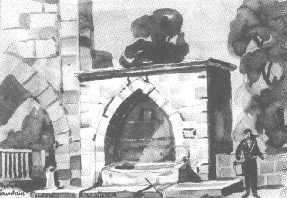
\includegraphics[scale=0.3]{atlas/cafer-fontana.png}
        &  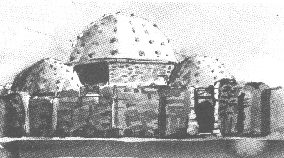
\includegraphics[scale=0.3]{atlas/cafer-bagno.png} \\
        1597 
        & 1601 \\
      \end{tabular}
    \end{center}
  }
  \only<2>{
    \begin{center}
      \begin{tabular}{p{0.48\textwidth}p{0.48\textwidth}}
        {\centering\includegraphics[scale=0.3]{documenti/vecellio295.png}}&
        {\centering\includegraphics[scale=0.4]{ritratti/Nadiri_f_8_v.jpg}}\\ 
        
        {\centering\tiny {\sc Cesare Vecellio}, {\it Habiti antichi et moderni
            di tutto il mondo}, Venezia, 1598}
        
        & {\centering\tiny
            {\it  Musicisti di fronte  a Mehmed  III}, Topkapı  Sarayı Müzesi,
            inv.  H889, f.  8, XVII  sec.} \\
      \end{tabular}
    \end{center}
  }

  \only<3>{
    \begin{center}
      \begin{tabular}{cc}
        \includegraphics[scale=0.25]{foto/aleppo-room-pergamon-1.png} &
        \includegraphics[scale=0.25]{foto/aleppo-room-pergamon-2.png} \\[1cm]
        \multicolumn{2}{c}{\tiny {\it Sala di Aleppo}, 1600-01, 
          Museums für Islamische Kunst (Pergamon), Berlin}\\ 
      \end{tabular}
    \end{center}
  }

}

\myincslide{frame:cafer}{2}
\myincslide{frame:cafer}{3}

\mode
<article>

Cafer Paşa si firma come  \RL{mIri mIrlar qubris}, {\it Mîr-i mîrler-i
  Kıbrıs},  ossia governatore di  Cipro. In  realtà, lui  stesso nella
lettera dice di esserlo stato in passato, lasciando sottindere che non
lo è più in questo momento.

Cafer  Paşa sarà  comunque spesso  governatore di  Cipro negli  anni a
cavallo  del  1600 (dal  1003/1595  al  1038/1629),  anche in  periodi
successivi  a  questa  lettera   \cite[p.  9]{sengor}.  A  Cipro  farà
costruire  tra   le  altre  cose   un  bagno  (1601)  e   una  fontana
(1597). Muore intorno al 1620.

Il  termine consueto  per  governatore sarebbe  \RL{mIri mIrAn},  {\it
  Mîr-i mîran}  \cite[p. 6]{sengor}. Tuttavia qui, come  in altri casi
all'interno della lettera,  Cafer Paşa non usa il  plurale persiano in
\RL{BAn}, {\it -an}, ma quello turco in \RL{Blar}, {\it -lEr}.

Da notare che il dragomanno traduce il titolo con Beylerbey.

\mode
<all>

\myframet{Muhibbane inha}{Inha}{frame:muhibbane}{

  \mbox{ }
  \vfill

  \parbox[c]{0.4\textwidth}{
    \begin{tabular}{c}
      \includegraphics{parole/muhibbane.png}\\
      \RL{mu.hibbAnah  in.hA}\\[1cm]
      muhibbane inha\\[1cm]
    \end{tabular}}
  \hfill
  \parbox[c]{0.55\textwidth}{
    \begin{tabular}{c}
      \includegraphics[scale=0.1]{documenti/frammento.png}\\[2mm]
      {\tiny ASVE, {\it Documenti Turchi}, n. 1099}\\[1cm]
      \includegraphics[scale=0.1]{documenti/doc1050.png}\\[2mm]
      {\tiny ASVE, {\it Documenti Turchi}, n. 1050}\\[1cm]
    \end{tabular}}

  \vfill
}

\myframe{Venedik Duzı}{frame:venedikduzi}{

\setarab
\novocalize
\begin{center}
\begin{tabular}{lr}
  \multicolumn{2}{c}{\includegraphics{parole/venedik_duzi.png}}\\
  Venedik duzı & \RL{wenedIk dUzI}\\[1cm]
  \multirow{2}{*}{\includegraphics[scale=0.28]{ritratti/marino_grimani.jpg}}&
    Marino Grimani\\
    &1532-1605, doge dal 1595\\[2cm]
    &\parbox{0.3\textwidth}{\tiny Gabriele Caliari, {\it Il doge Marino Grimani riceve l'ambasciatore persiano}, Venezia, Palazzo Ducale, XVI sec.}\\
\end{tabular}
\end{center}
\setfarsi
}

\mode
<article>

Cafer Paşa scrive al Doge di Venezia, all'epoca Marino Grimani.\cite{itmarinogrimani}

\mode
<all>

\myframe{Kıbrıs}{frame:kibris}{
\setarab
\novocalize
\begin{center}
\begin{tabular}{l@{\hspace{2cm}}r}
  \multicolumn{2}{c}{\includegraphics{parole/kibris_vilayet.png}}\\
  bu muhibları vilâyet Kıbrıs
  & \RL{bU mu.hiblarY wilAyat qubris}\\[1cm]
  \multicolumn{2}{c}{
    \parbox[c]{0.58\textwidth}{\centering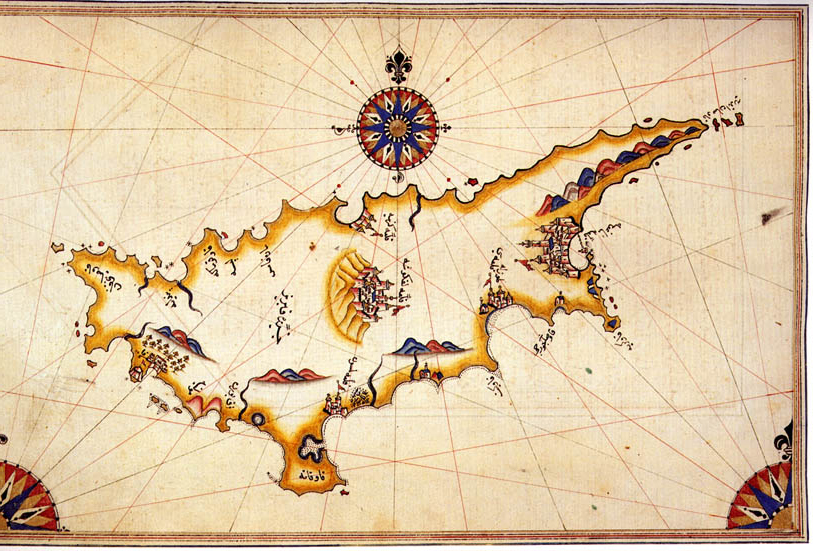
\includegraphics{atlas/Cyprus_by_Piri_Reis.jpg}}
    \parbox[c]{0.35\textwidth}{\tiny {\sc Piri Reis}, {\it Kitab-ı Bahriye}, 1521-25}}\\
\end{tabular}
\end{center}
}

\myframe{Yaqumu Biazii}{frame:yaqumu}{
\setfarsi
\novocalize
\parbox[c]{0.48\textwidth}{
  \begin{tabular}{c}
    \includegraphics{parole/yaqum_biazii.png}\\
    \RL{yaqumU byAzY nAm}\\
    Yaqumu Biazii nam\\[0.5cm]
    \includegraphics{parole/rayetinize.png}\\
    \RL{ra`iyatikizah}\\
    ra`iyetinize\\
\end{tabular}}\hfill\parbox[c]{0.5\textwidth}{\centering
  \begin{tabular}{p{0.48\textwidth}}
    \includegraphics[scale=0.3]{documenti/vecellio321.png}
    \includegraphics[scale=0.3]{ritratti/mercante2.png}\\[0.2cm]
    {\tiny {\sc Cesare Vecellio}, {\it Habiti antichi et moderni di tutto il mondo}, Venezia, 1598}\\
  \end{tabular}}
}

\mode
<article>

Nella lettera racconta che,  quand'era a Cipro come governatore, aveva
conosciuto  un tal  \RL{yaqumU  byAzY}, {\it  Yaqumu Biazii}  (Giacomo
Biasii), nel quale  lui riponeva fiducia. Questo Biasii  è indicato al
doge  come \RL{ra`iyatikizah},  {\it ra`iyetinize},  cioè  {\it vostro
  suddito}. Si tratta quindi di un veneziano.

\mode
<all>

\myframe{Penbe}{frame:penbe}{
  \setfarsi
  \novocalize
  \parbox[c]{0.4\textwidth}{\centering\begin{tabular}{c}
      \includegraphics{parole/penbe.png}\\[1cm]
      \RL{panbah}\\[1cm]
      penbe\\
  \end{tabular}}
  \hfill\parbox[c]{0.55\textwidth}{
    \begin{tabular}{c}
      \includegraphics[scale=0.6]{documenti/alpino.jpg}\\
      {\tiny {\sc Prosper Alpinus}, {\it De Plantis Aegypti Liber}, Venezia 1592}\\
  \end{tabular}}
}

\myframet{Agnello vegetale}{A. vegetale}{frame:agnellovegetale}{
  \setfarsi
  \novocalize
  \tiny
  \begin{tabular}{cp{0.5\textwidth}}
    \includegraphics[scale=0.5]{documenti/Mandeville_cotton.jpg}&
    {\centering\includegraphics[scale=0.15]{documenti/Vegetable_lamb.jpg}}\\[0.4cm]
    Jehan  de Mandeville, 1357-1371 & {\centering  Johann Zahn's, {\it
        Specula Physico-Mathematico-Historica Notabilium ac Mirabilium
        Sciendorum}, Norinberga, 1696}\\
  \end{tabular}
}

\myframe{Kıbrıs kantar}{frame:kantar}{
  \setfarsi
  \novocalize
  \begin{center}
    \begin{tabular}{c}
      \includegraphics{parole/kantar.png}\\[0.5cm]
      \RL{qubris  qan.tArIlah  saksAn  bi^s  qan.tAr wa  awn  .tuqUz  ludraH lar}\\[0.5cm]
      Kıbrıs kantarıla  seksen beş kantar  ve on  dokuz lodralar\\
    \end{tabular}
  \end{center}
}

\myframe{Çuval}{frame:cuval}{
  \setfarsi
  \novocalize
  \parbox[c]{0.5\textwidth}{\centering\begin{tabular}{c}
      \includegraphics{parole/cuval.png}\\[1cm]
      \RL{saksAn  bir qi.ta`ah  ^cuwAl}\\[1cm]
      seksen bir kıt'a-ı çuval\\
  \end{tabular}}
  \hfill\parbox[c]{0.4\textwidth}{
    \begin{tabular}{c}
      \includegraphics[scale=0.3]{documenti/luzerner.png}\\
      {\tiny {\sc Diebold Schillieg}, {\it Luzerner Chronik}, 1517}\\
  \end{tabular}}
}

\myframe{Sikke}{sikke}{
  \begin{center}
  \begin{tabular}{c}
    \includegraphics{parole/sikke.png}\\[0.2cm]
    \RL{iw^c {\setarab  bIk} {\setverb yadI} yUz  sikkah  altUnliq panbah}\\[0.2cm]
    üç  bin  yedi  yüz  sikke altınlık\\[0.5cm]
    \includegraphics{monete/sanmatteo.png}\\[0.2cm]
    {\tiny Caravaggio, {\it Vocazione di San Matteo}, 1599-1600}\\
  \end{tabular}
  \end{center}
}



\mode
<article>

Si tratta di cotone, stimato 3700  monete d'oro, in 81 sacchi del peso
di 85 cantara e 19 lodra.

\mode
<all>

\myframe{Venediğe}{frame:venedige}{
\setarab
\novocalize
\begin{center}
\begin{tabular}{c}
  \includegraphics{parole/venedikte.png}\\[0.2cm]
  \RL{wanadIkah  alUb kIdUb bay`i {\setarab iytmak}  iy^cUn}\\[0.2cm]
  Venediğe alup gidup beyi etmek  içün\\[0.5cm]
  \includegraphics[scale=0.2]{atlas/venezia.png}\\
  {\tiny Bolognino Zaltieri, 1565}\\
\end{tabular}
\end{center}
}

\mode
<article>

Siccome appunto si fidava di  questo Biasii, gli aveva dato della merce
da vendere a Venezia.

\mode
<all>

\myframet{Il viaggio del cotone}{V. cotone}{frame:viaggiocotone}{
  \begin{center}
    \includegraphics[scale=0.3]{atlas/viaggio-cotone.png}
  \end{center}
}

%\mysection{Il cotone a Venezia}

\frameturcodocslice{Murd veresesi}{verese}{verese}
                   {murd  mizbUrik  wara_tah  {\setarab  sI}}  
                   {murd-i  mezburin veresesi}

\frameturcodocslice{Marco d'Aldi}{marcodaldi}{marco_daldi}
                   {mArqU  dah  {\setarab   aldI}  nAm}
                   {Marco d'Aldi nam}

\mode
<article>

Succede che Biasii muore durante il viaggio. Quando il carico arriva a
Venezia, viene incamerato insieme ai beni del morto, e adesso si trova
nelle mani o degli eredi oppure di un certo Marco d'Aldi.

\mode
<all>

\myframet{Girolamo Cappello}{Cappello}{frame:cappello}{
\setarab
\novocalize
\only<1>{\turcodocslice{capello}
                   {astAnaH-e dawlat madAradaH bAylUs awlAn ^sukUr qAbilU nAm}
                   {Asitane-i devletmedarda baylos olan şükur Kabilu nam}}
\only<2>{\begin{center}
\begin{tabular}{p{0.6\textwidth}p{0.35\textwidth}}
  {\centering\includegraphics[scale=0.3]{documenti/udienza.png}}&
  {\centering\includegraphics[scale=0.2]{ritratti/S21B4-2SII_00_il9_440x690.jpg}}\\  {\centering\tiny {\it  Un'udienza alla corte ottomana}, 1586, Österreichische Nationalbibliothek, Wien, cod. 8615, f. 134v}  & 
 {\centering\tiny {\it  Selim II
      riceve l'ammbasciatore austriaco},
    Topkapı Sarayı Müzesi, inv. H1339, f. 178, 1568-69}\\
\end{tabular}
\end{center}}
}

\myincslide{frame:cappello}{2}

%{ritratti/Nehzetul-Ahbar_der_Sefer-i_Sigetvar_247b.jpg}
%{\centering\tiny {\it  Selim II
%      riceve l'ammbasciatore safavide al  palazzo di Edirne nel 1567},
%    Topkapı Sarayı Müzesi, inv. H1339, f. 247b, 1568}

\mode
<article>

Cafer  Paşa  lo   sa  perché  si  è  rivolto   al  bailo  veneziano  a
Costantinopoli, Cappello,  il quale  ha chiesto informazioni  a Venezia
sulla faccenda.

Dopo   aver   chiesto   queste   informazioni,  Cappello   rientra   a
Venezia. Siccome Cappello  termina il mandato nel 1599  e relaziona al
Senato il 26  febbraio 1600, si può datare la lettera  tra la fine del
1599 e l'inizio del 1600 \cite{pedani2002}.

\mode
<all>

\frameturcodocslice{Cinqu Savii}{cinqusavii}{cinqu_savii}
                   {^cinqU   {\setarab  sAwI}   nAm  {\setarab baklarik}}
                   {Cinqu Savii nam beylerin}

\mode
<article>

Il bailo  dice a Cafer Paşa  di presentare la vicenda  ai Cinque Savii
alla Mercatura a Venezia.

\mode
<all>

\myframe{Procuratore}{frame:procuratore}{
  \setfarsi
  \novocalize
  \begin{center}
    \begin{tabular}{c}
      \includegraphics{parole/procuratore.png}\\[1cm]
       \RL{`aliyh kimisnah wakIl na.sb wa ta`yIn} \mancante{} \RL{bir} \\[1cm]
      bir \mancante{}  aleyhe kimesne vekil nasp ve ta`yın [et-/olun-]\\
    \end{tabular}
  \end{center}
}

\mode
<article>

Il bailo gli aveva suggerito di  nominare un uomo di fiducia a Venezia
che si occupasse dei suoi interessi.

Quest'espressione,  che letteralmente  significa  {\it designazione  e
  nomina di un qualche agente verso ???}, è usata due volte
nel testo, una con {\it et-} e una con {\it olun-}. In entrambi i casi
il senso è {\it nominare un procuratore}.

\mode
<all>

\myframe{Çavuş}{frame:cavus}{
  \setfarsi
  \novocalize
  \only<1>{
    \begin{center}
      \begin{tabular}{c}
        \includegraphics{parole/gondermeki.png}\\[1cm]
        \RL{bir ^cAwu^s kUndarmakY}\\[1cm]
        bir çavuş göndermeği\\
      \end{tabular}
    \end{center}
  }
  \only<2>{
    \begin{center}
      \begin{tabular}{c}
        \includegraphics{parole/gonderilmiyub.png}\\[1cm]
        \RL{^cAwu^s kUndarilmIwb}\\[1cm]
        çavuş gönderilmiyüb\\
      \end{tabular}
    \end{center}
  }
}


\myincslide{frame:cavus}{2}

\mode
<article>

Inizialmente, Cafer Paşa aveva pensato  di inviare un çavuş a Venezia.
Ma il  bailo l'aveva dissuaso,  dicendogli che era meglio  nominare un
procuratore, invece di inviare qualcuno.

In  questo  Cappello  ha  seguito  le  disposizioni  del  Senato,  che
invitavano i  baili a scoraggiare  il più possibile l'invio  di çavuş,
che  dovevano essere  spesati  dalla Repubblica  nel  viaggio e  nella
permanenza a Venezia, oltre che ricevere regali \cite{pedani1994}.

\mode
<all>

\frameturcodocslice{Abodinti}{abodinti}{abodinti}
                   {{\setarab   abUdIntI}  nAm   yahUdIler}
                   {Abodinti nam yahudiler}%16

\frameturcodocslice{Musa Magiaod}{musamagiaod}{musa_magiaod}
                   {nafs wanidIkdah  awlAn mUsA  ma^gA|Awd  nAm}
                   {nafs Venedikte olan Musa Magiaod nam}%17

\mode
<article>

Cafer Paşa  si rivolge quindi agli Abodinti  (Abondanti), una famiglia
ebrea con  cui era in rapporti,  e chiede di poter  utilizzare il loro
agente a Venezia, l'ebreo Musà  Magiaod. Loro accettano e quindi Cafer
Paşa lo nomina suo procuratore.

Quindi questa è la lettera d'incarico di Musà Magiaod.

\mode
<all>

\myframe{Bir barça ile}{frame:barca}{
  \parbox[c]{0.6\textwidth}{
    \turcodocslice{barca}{bir bAr^cah iylah}{bir barça ile}
  }\hfill\parbox[c]{0.35\textwidth}{
    \begin{tabular}{p{0.34\textwidth}}
      \includegraphics[scale=0.3]{navi/birbarca.png}\\
                      {\tiny Bolognino Zaltieri, 1565}\\
    \end{tabular}
  }
}

\myframe{Sınguriye}{frame:senguriye}{
  \setfarsi
  \novocalize
  \begin{center}
    \begin{tabular}{c}
      \includegraphics{parole/singuria.png}\\[1cm]
      \RL{bizim  nAmimizah .sin.gUryah iydUb}\\[1cm]
      bizim namımıza sınguriye edup\\
      %\visible<3->{se(n)gur}\visible<2->{-iye}\\
    \end{tabular}
  \end{center}
}


\mode
<article>

Musà Magiaod è incaricato da Cafer  Paşa di recuperare il denaro che è
stato riscosso per la vendita del cotone e tutto quanto avanza secondo
un certo inventario che dice di aver già mandato.

Il  tutto dovrà essere  imbarcato su  una qualche  nave e  andrà fatta
l'assicurazione a nome di Cafer Paşa.

\mode
<all>



\mysection{Il periodo}

\myframe{Alcuni avvenimenti del 1600}{frame:1600}{
  \input{frame/lineadeltempo}
}

\myframe{Principali rotte commerciali nel XV-XVII secolo}{frame:prescoperte}{
  \begin{center}
  \includegraphics{atlas/economiamondoprescoperte.png}
  \end{center}
}

\myframe{L'economia mondo nel 1500}{frame:ecomondo1500}{
  \begin{center}
  \includegraphics[scale=2]{atlas/economiamondo1500.png}
  \end{center}
}

\myframe{L'economia mondo nel 1750}{frame:ecomondo1750}{
  \begin{center}
  \includegraphics[scale=2]{atlas/economiamondo1750.png}
  \end{center}
}




\mode
<article>

\newpage

\mode
<all>

\mysection{La quantità}

\myframe{Unità di misura}{frame:unitamisura}{
  \begin{center}
    \begin{tabular}{rl}
      \includegraphics[scale=0.15]{documenti/Bilancioimg-000.png}
      &\includegraphics[scale=0.15]{documenti/Bilancioimg-001.png}
    \end{tabular}
  \end{center}
}


\myframe{Conversione}{frame:conversione}{
  \begin{center}
    {\color{evidenzia}\bf 85 cantara di Cipro e 19 lodra}
    
    \vfill
    
    \only<1>{\scriptsize
      \rule[-1em]{0pt}{6cm}\begin{tabular}[b]{rcccl}
        1 &cantara di Cipro &$\cong$& 750 &libbre sottili veneziane\\
        1 &libbra sottile veneziana&$\cong$& 300 &g\\
        1 &cantara &$\cong$ &225 &kg \\[1cm]
        1 &cantara &$=$&44& okka\\
        1 &okka&$=$&4& lodra\\
        1 &cantara&$=$&176& lodra\\[0.5cm]
        {\it oppure}\\[0.5cm]
        1 &cantara&$=$&100& rotoli\\
        1 &rotolo&$=$&1& lodra\\
        1 &cantara&$=$&100& lodra\\
      \end{tabular}
    }
    \only<2>{\scriptsize
      \rule[-1em]{0pt}{6cm}\begin{minipage}[b]{\textwidth}
        \begin{eqnarray*}
          85\,\text{cantara} + 19\, \text{lodra} 
          &=& 85+\frac{19}{176}\, \text{cantara} \\
          &=& \left(85+\frac{19}{176}\right)225\, \text{kg}\\
          &=& 19149.29\, \text{kg} \cong 20\,\text{t}\\[1cm]
          85\,\text{cantara} + 19\, \text{lodra} 
          &=& 85+\frac{19}{100}\, \text{cantara} \\
          &=& \left(85+\frac{19}{100}\right)225\, \text{kg}\\
          &=& 19167.75\, \text{kg} \cong 20\,\text{t}
        \end{eqnarray*}
      \end{minipage}
    }
  \end{center}
}

\myincslide{frame:conversione}{2}

\mode
<article>

Per  stimarne  il  peso  in  chilogrammi, utilizziamo  un  manuale  di
commercio del  XVIII secolo. Questo manuale  è più tardo  di circa 150
anni, ma  il valore indicato per  il cantara è coerente  con quello di
altre fonti \cite[p. 40]{triulzi1766}.

Secondo questo manuale,  un cantara di Cipro corrisponde  a 750 libbre
sottili veneziane.   Una libbre sottile veneziana varia  a seconda del
periodo intorno ai 300 g (301.2 g), quindi il cantara di Cipro sarebbe
più o meno 225 kg \cite{websizes}.

Per quanto rigurda la lodra, può  essere intesa in due modi. In alcuni
casi è un  sinonimo del rotolo e quindi corrisponde  a un centesimo di
cantara \cite{websizes}. In  altri casi è un quarto  di un'okka, che a
sua volta è un quarantaquattresimo di cantara, il che dà 176 lodra per
cantara \cite[voce {\it lodra}]{okyanus}.

Questo valore è  comunque ininfluente, dato che in  entrambi i casi si
arriva ad una stima di poco meno di 20 tonnellate.

La  parola   lodra  è  formata   sull'arabo  {\it  rotl}   (rotolo)  e
sull'italiano {\it libra} \cite[voce {\it lodra}]{okyanus}.

\mode
<all>

\myframe{I sacchi}{frame:sacchi}{
  \begin{center}
    {\color{evidenzia}\bf 81 sacchi}
    
    \vfill
    
    \parbox[c]{0.5\textwidth}{\centering
      \begin{equation*}
        \frac{20\,\text{t}}{81\,\text{sacchi}}\cong 247 \,\text{kg per sacco}
      \end{equation*}
    }
    \hfill\parbox[b]{0.4\textwidth}{
      \begin{tabular}{c}
        \only<1>{\cparbox{0.38\textwidth}{6cm}{\includegraphics[scale=0.3]{documenti/luzerner.png}}}
        \only<2>{\cparbox{0.38\textwidth}{6cm}{\includegraphics[scale=0.4]{documenti/luzerner-sacco.png}}}\\
                {\tiny {\sc Diebold Schillieg}, {\it Luzerner Chronik}, 1517}\\
    \end{tabular}}
  \end{center}
}

\myincslide{frame:sacchi}{2}

\myframe[3]{Il volume del cotone}{frame:dimensione}{
  \begin{center}
    \input{frame/camioncotone}
  \end{center}
  
  {\footnotesize
    {\it Bales  of cotton being  transported from  Bakersfield to  the cotton
      compress on Terminal Island}, 
    ca. 1932,
    Long Beach Public Library,
    Long Beach, California}
}

\mode
<article>

La dimensione  delle balle  che si vedono  nella riproduzione  è molto
simile a quelle di questa foto.  Nella foto ci sono circa 70 balle, un
valore molto vicino a quello della lettera.

\mode
<all>

\myframe{Galeone veneziano}{frame:galeone}{
  \begin{center}
    \parbox[c]{0.7\textwidth}{\includegraphics[scale=0.8]{navi/santissimamadre.png}}
    \hfill
    \parbox[c]{0.28\textwidth}{\tiny {\it Santissima Madre}, Venezia, circa 1550}
  \end{center}
}

\mode
<article>

Da \cite[p. 48]{cucari2004}

Generalmente, i grossi traffici veneziani avvengono con navi di grosso
dislocamento  (722 t).  Tuttavia,  alla fine  del  secolo (dal  1573),
nessuno è più in grado di  costruire una nave del genere senza l'aiuto
dello stato \cite[p. 325]{braudel1982}.

\mode
<all>

\myframe{Marciliana}{frame:marciliana}{
  \begin{center}
  \includegraphics[scale=0.4]{navi/marciliana.png}
  \end{center}
}

\mode
<article>

Compaiono quindi navi  di stazza più piccola, sulle  150 t, dette {\it
  marciliane}. Ma l'incapacità (o la  non volontà) di Venezia a varare
più  navi  di  questo  tipo  favorisce la  navi  Francesi,  Inglesi  o
Olandesi.  Questi  mercanti ``stranieri'' invadono  i porti e  sono in
grado  di pagare  di più  le merci,  anche lo  stesso cotone  di Cipro
\cite[p. 329]{braudel1982}.

\mode
<all>

\myframe{Susan Constant}{frame:susanconstant}{
  \begin{center}
    \includegraphics{navi/susanconstant.png}

    \vspace{1cm}

    {\tiny {\it Susan Constant (ricostruzione)}, London, 1605}
  \end{center}
}

\myframe{Mary Rose}{frame:maryrose}{
  \begin{center}
  \input{frame/maryrose.tex}

  {\tiny {\it Mary Rose}, Portsmouth, 1511}
  \end{center}
}

\mode
<article>

Mary     Rose:    da     \cite[p.     97]{marsden2003}    (foto)     e
\cite[p. 93]{marsden2003} (disegno).

Susan Constant: da \cite[p. 88]{lavery2005}.

\mode
<all>




\mode
<article>

\newpage

\mode
<all>

\mysection{Il valore}

\myframe{Altun}{frame:altun}{
  \begin{center}
    \begin{tabular}{c}
      \includegraphics{monete/marino_grimani.jpg}\\
      {\it ducato veneziano} coniato sotto Marino Grimani (1595-1605)\\
      22 mm, 3.50 g, 500 \EUR\\[0.5cm]
      \includegraphics[scale=0.25]{monete/sultani_mehmedIII.png}\\
      {\it sultanî} coniato ad Amasya sotto Mehmed III (1003/1597) \\
      19-22 mm, 3.28-3.50 g\\
    \end{tabular}

  \end{center}
}

\mode
<article>

Nella slide si vedono due  monete d'oro contemporanee alla lettera. La
prima è un ducato veneziano, la seconda un sultanî.

La prima immagine è tratta dal  sito di una casa d'aste, che valuta la
moneta 500 \EUR. I valori di diametro e peso sono quelli della moneta.

La  seconda da  un  sito di  numismatica  ottomana, per  cui i  valori
indicano  il  range che  poteva  avere  questa  moneta.  Gli  ottomani
coniavano  monete  in  più  zecche  sparse  per  l'impero.  Questa  in
particolare viene da Amasya.

\mode
<all>

\myframe{Akçe}{frame:akce}{
  \footnotesize
  \begin{center}
    \begin{tabular}{p{0.48\textwidth}p{0.48\textwidth}}
      {\centering\includegraphics[scale=0.25]{monete/13-1003-dirhem-haleb.png}}&
      {\centering\includegraphics[scale=0.25]{monete/akce2.png}}\\
      {\centering{\it dirhem} coniato a Aleppo sotto Mehmed III (1003/1597), 19 mm, 2.02-2.70 g} &
      {\centering{\color{evidenzia}\it akçe} coniato a Cipro sotto Mehmed III (1003/1597),
        11 mm, 0.35 g}\\
      {\centering 100 dirhem = 800 akçe} & {\centering 1 altun = 120 akçe} \\[5mm]
    \multicolumn{2}{c}{\includegraphics[scale=0.25]{monete/1587-8reales-felipe2-segovia.jpg}}\\
    \multicolumn{2}{c}{{\it real de a ocho} coniato in Spagna sotto Filippo II (1597), 40 mm, 27.2 g}\\
    16 real = 1 altun & 2 real de a ocho = 1 altun \\
    
    \end{tabular}
  \end{center}
}

\mode
<article>

Per  avere  un'idea  del  valore  di 3700  monete  d'oro,  è  comunque
necessario   cercare  un'equivalenza  con   il  valore   delle  monete
d'argento, dato che salari, prezzi  e bilanci erano espressi in questa
unità di misura.

In questo momento, nell'impero ottomano  si usa due tipi di monete: la
moneta d'oro ({\it altun}), usata  per gli scambi internazionali, e la
moneta d'argento ({\it akçe}), usata invece per le spese correnti.

Mentre l'{\it altun}  ha una quantità d'oro e  un valore relativamente
stabile  nel tempo e  uniforme nel  Mediterraneo, la  moneta d'argento
subisce una forte e veloce svalutazione a partire dall'inizio del XVI.
Questo fenomeno  è chiamato {\it  Rivoluzione dei prezzi}  e colpisce,
anche se in modo diverso, tutto  il mondo europeo in senso molto largo
\cite{braudel1982,barkan1975,pamuk2001}.

\mode
<all>

\myframe{La svalutazione delle monete d'argento}{frame:svalargento}{
  \includegraphics[scale=0.9]{schemi/svalutazione.png}
}

\myframe[5]{Il valore del cotone in akçe}{frame:valakce}{
  \begin{center}
    \begin{tabular}{>{\it}rccccc|ccc}
     &&&&&& \multicolumn{3}{l}{3700 monete d'oro}\\[1cm]
     \visible<2-6>{ufficiale} & \visible<2-6>{1} & \visible<2-6>{altun} & \visible<2-6>{=} & \visible<2-6>{120} & \visible<2-6>{akçe} & 
     \visible<3-6>{=} &\visible<3-6>{444\hspace{0.2em}000} & \visible<3-6>{akçe}\\[1cm]
     \visible<4-6>{reale} & \visible<4-6>{1} & \visible<4-6>{altun} & 
     \visible<4-6>{$\cong$} & \visible<4-6>{180} & \visible<4-6>{akçe}&  
     \visible<5-6>{=} & \visible<5-6>{666\hspace{0.2em}000} & \visible<5-6>{akçe}\\[1cm]
    \end{tabular}

    \vspace{1cm}

    \visible<6>{ {\it Narh Defteri}, 15 novembre 1600 } 
  \end{center}
}

%\myincslide{frame:valakce}{5}

\mode
<article>

Negli anni tra il 1585 e il 1599, il valore dell'{\it akçe} continua a
calare drammaticamente e soprattutto  si discosta dal valore ufficiale
di cambio \cite[p. 12-14]{barkan1975}.

L'amministrazione interverrà il 15 novembre  del 1600 con il {\it Narh
  Defteri}, che regola il  valore dell'{\it akçe} e contemporaneamente
il prezzo delle merci, riportando il valore di cambio a 120 {\it akçe}
per un  {\it altun}  \cite[p. 13]{barkan1975}. Quest'evento  è tuttavia
successivo al documento.

\mode
<all>

\myframe[4]{Indice dei prezzi}{frame:indice}{
  \begin{center}
    \input{frame/indiceprezzi}

    {\footnotesize  Indice dei prezzi  delle vettovaglie  dai registri
      degli {\it imaret}, 1490-1655. La  linea solida è in {\it akçe},
      quella tratteggiata in grammi d'argento.}
  \end{center}
}

\mode
<article>

Il grafico  è una rielaborazione  da \cite[p. 15]{barkan1975}.  I dati
dell'argento vengono rivisti al ribasso in \cite[p. 80]{pamuk2001}.

\mode
<all>

\def\coldue{\only<2->{\color{evidenzia}}}

\myframe[4]{Salari degli operai edili}{frame:salari}{
  \begin{center}
    \begin{tabular}{r*{4}{r@{.}l}}
      \hline
      \multicolumn{9}{c}{\bf Salari giornalieri}\\
      \hline
      &\multicolumn{4}{c}{non esperti} & \multicolumn{4}{c}{esperti}  \\
      anni & \multicolumn{2}{c}{akçe} & arg& (g)  
      & \multicolumn{2}{c}{akçe} & arg& (g) \\
      \hline
      1580-1589 &  8&1 & 3&5 & 12&4 & 5&4 \\
      \coldue 1590-1599 &\coldue  11&\coldue 7 &\coldue  2&\coldue 6 &\coldue  20&\coldue 7 &\coldue  4&\coldue 6 \\
      \color{black}1600-1609 & 13&9 & 4&0 & 22&5 & 6&5 \\
      \hline
    \end{tabular}

    \vspace{1cm}

    \visible<3->{\parbox[8]{0.6\textwidth}{Operaio esperto all'anno (su 200 giorni) nel periodo 1590-1599:}\hfill 4140 akçe}

    \vspace{1cm}

    \visible<4->{Con 8-12 akçe: 8 kg di pane o 2.5 kg di riso o 2 kg di montone} 

  \end{center}
} 

\mode
<article>

Il grafico viene da \cite[p. 301]{ozmucur2002}.

All'epoca di Süleyman, l'{\it  ağa} dei Giannizzeri aveva una pensione
di 300 akçe al giorno e un alto  ufficiale tra i 120 e i 150, oltre ad
alloggio,    parte    del    vitto    e    parte    dell'abbigliamento
\cite[p. 191]{horniker1944}.

In  ogni caso, la  paga di  un operaio  esperto gli  consentiva, anche
lavorando meno di  duecento giorni l'anno, di avere  un buon tenore di
vita \cite[p. 306-7]{ozmucur2002}.

\mode
<all>

\myframe{Prezzi di alcune merci}{frame:alcunemerci}{
  \small
  \begin{center}
    \begin{tabular}{>{\it}lcc}
      & prima del & dopo il \\
      &{\it Narh Defteri} 
      &{\it Narh Defteri}  \\
      & (in akçe) & (in akçe)  \\
      \hline
      100 {\it dirhem} di pane & 0.87 & 0.50  \\
      100 {\it dirhem} di pane di alta qualità & 1.25  & 0.83  \\
      1 {\it kile} di farina & 120 & 80  \\
      1 {\it kile} di farina di bassa qualità & 75 & 50  \\
      1 {\it kile} di riso & 56 & 39  \\
      1 {\it okka} di miele & 20 & 13 \\
      1 {\it okka} di burro & 26 & 19 \\
      1 cubito di velluto fine francese & 1200 & 550 \\
      1 cubito di velluto genovese & 880 & 400 \\
      1 cubito di lana pesante {\it nev-peyda} & 300 & 120 \\
      \hline
    \end{tabular}
  \end{center}

  \vspace{0.5cm}

  {\footnotesize
  \begin{tabular}{rcccl@{\hspace{1cm}}rcccl}
    100 & dirhem & $\cong$ & 300 & g &
    1 & kile   & $\cong$ & 36 & l \\
    1 & okka   & $\cong$ & 1.2 & kg &
               && $\cong$ & 10 & kg di farina \\ 
    1 & cubito & $\cong$ & 45 & cm &
               && $\cong$ & 15 & kg di riso \\ 
  \end{tabular}
  }
}

\mode
<article>

Da \cite[p. 13-14]{barkan1975}.

\mode
<all>

\myframe{Andamento dei salari}{frame:trend}{
  \begin{center}
  \input{frame/salari}
  \end{center}
}

\mode
<article>

Da  \cite[p.  306]{ozmucur2002}.   L'andamento dei  salari  continua a
calare e bisognerà aspettare il 1850 perché i salari tornino ai valori
del 1500.

A differenza di quanto succede  in occidente, dove è ancora largamente
diffuso il  baratto e  il pagamento in  natura (anche  delle imposte),
nell'impero  ottomano  l'uso  della   moneta  è  molto  diffuso  nella
popolazione urbana e in larghe  fasce di quella rurale. Quindi il calo
relativo  dei salari,  l'aumento dei  prezzi e  la  svalutazione della
moneta  hanno   un  impatto   enorme  virtualmente  su   tutti  quanti
\cite[p. 307-8]{ozmucur2002}.

Il problema è  se possibile maggiore per chi  ha uno stipendio fissato
per  legge  (soldati, impegati  dell'amministrazione,  ecc.). E'  però
anche  per  questo che  le  politiche  finanziare  come il  {\it  Narh
  Defteri} hanno successo.

\mode
<all>

\myframe[3]{Il prezzo della seta grezza a Bursa}{frame:prezzoseta}{
  \begin{center}
    \begin{tabular}{rr@{.}l}
      1595 & 197&06 \\
      \coldue 1597 & \coldue 224&\coldue 79 \\
      1603 & 351&05 \\
      1607 & 233&05 \\
    \end{tabular}

  \vspace{0.4cm}
  
  in {\it akçe} per {\it lodra}

  \vspace{1cm}
  \visible<3->{
    \begin{tabular}{rcccl}
      1 & cantara &$=$&176&lodra \\
      1 & cantara &$\rightleftarrows$&39\hspace{0.2em}563 &akçe\\[1cm]
      1 & cantara &$=$&100&lodra \\
      1 & cantara &$\rightleftarrows$&22\hspace{0.2em}479 &akçe\\
    \end{tabular}
  }
  \end{center}

}

\mode
<article>

Da \cite[p. 536]{cizakca1980}.

\mode
<all>

\myframe{Confronto}{frame:confronto}{
  \scriptsize
  \parbox[c]{0.4\textwidth}{\includegraphics[scale=0.15]{documenti/Bilancioimg-002.png}}
  \hfill\parbox[c]{0.55\textwidth}{
    \begin{center}
    \begin{tabular}{r>{\centering}p{1cm}ccp{1cm}}
      1 &cantara di Cipro &$\cong$& 750 &libbre sottili\\[2mm]
      1 &cantara di Bursa &$\cong$& 176 &libbre sottili\\[2mm]
      1 &cantara di Cipro &$\cong$& 4.26 &cantara di Bursa\\[4mm]
      85 & cantara di Cipro & $\cong$& 362 & cantara di Bursa\\[4mm]
      362 & cantara di Bursa di seta grezza & $\rightleftarrows$ 
      & 14\hspace{0.2em}321\hspace{0.2em}806 & akçe\\[2mm]
          &                                 & $\rightleftarrows$ 
      & 8\hspace{0.2em}137\hspace{0.2em}398 & akçe\\
    \end{tabular}

    \vspace{1cm}
    {\normalsize 444\hspace{0.2em}000 $\div$ 666\hspace{0.2em}000 akçe}
    \end{center}

  }
}



\mysection{Storia del cotone}

\myframe{Erodoto}{frame:erodoto}{

\textgreek{
τὰ δὲ δένδρεα τὰ ἄγρια αὐτόθι φέρει καρπὸν εἴρια καλλονῇ τε προφέροντα καὶ ἀρετῇ τῶν ἀπὸ τῶν ὀίων: καὶ ἐσθῆτι Ἰνδοὶ ἀπὸ τούτων τῶν δενδρέων χρέωνται.}

{\mbox{ }\hfill  Erodoto, {\it Storie, 3.106.3}, V sec. a.C.}

\vspace{1cm}

Laggiù le piante selvatiche producono come frutto una lana che supera
in bellezza e qualità quella delle pecore: e per le vesti gli Indiani
si riforniscono proprio con queste piante.

}

\myframe{Prospero Alpino}{frame:alpino}{
  \begin{tabular}{cp{5cm}}
    \multirow{3}{*}{\includegraphics[scale=0.65]{documenti/alpino.jpg}}&
    {\sc Prosper Alpinus},\\& {\it De Plantis Aegypti Liber},\\& Venezia 1592\\[6cm]
  \end{tabular}
}

\myframet{Agnello vegetale}{A. vegetale}{frame:agnellovegetale}{
  \setfarsi
  \novocalize
  \tiny
  \begin{tabular}{cp{0.5\textwidth}}
    \includegraphics[scale=0.5]{documenti/Mandeville_cotton.jpg}&
    {\centering\includegraphics[scale=0.15]{documenti/Vegetable_lamb.jpg}}\\[0.4cm]
    Jehan  de Mandeville, 1357-1371 & {\centering  Johann Zahn's, {\it
        Specula Physico-Mathematico-Historica Notabilium ac Mirabilium
        Sciendorum}, Norinberga, 1696}\\
  \end{tabular}
}

\myframet{Il viaggio del cotone}{V. cotone}{frame:viaggiocotone}{
  \begin{center}
    \includegraphics[scale=0.3]{atlas/viaggio-cotone.png}
  \end{center}
}


%% \myframe{Sacchi}{frame:sacchi}{
%%   \begin{tabular}{p{\textwidth}}
%%     \includegraphics[scale=0.3]{navi/lavoratoriporto.jpg}\\  {\it Lavoratori del
%%       porto di  Genova tra  sacchi di cotone  (a sinistra) e  balle di
%%       lane  (a destra)}, fine 800\\
%%   \end{tabular}
%% }

%% \myframe{Cotone imbarcato}{frame:imbarcato}{
%%     \begin{center}
%%       \input{frame/cotoneimbarcato}
%%       {\it Bales of cotton on a steamboat dock ready for shipping}
%%     \end{center}
%% }


\mode
<article>

\newpage

\mode
<all>

\mysection{Appendice}

\myframet{L'Europa nel 1600}{Europa 1600}{frame:europa1600}{
  \begin{center}
    \includegraphics[scale=0.25]{atlas/europe_map_1600.jpg}
  \end{center}
}

\myframet{Le company inglesi}{Companies}{frame:companies}{
  \begin{center}
    \includegraphics[scale=1.5]{atlas/companies-ok.png}
  \end{center}
}

\myframet{Il commercio veneziano}{Commercio}{frame:commveneziano}{
  \begin{center}
    \includegraphics[scale=0.25]{atlas/Repubblica_di_Venezia.png}
  \end{center}
}

\myframet{L'economia mondo dei romani}{Romani}{frame:ecoromani}{
  \begin{center}
    \includegraphics{atlas/romani-ok.png}
  \end{center}
}

\myframe{La tessitura}{frame:tessitura}{
  \begin{center}
    \includegraphics[scale=0.45]{documenti/269tessitore.jpg}
  \end{center}
}

\myframet{Polizza del 1404}{Polizza 1404}{frame:polizza1404}{
  \begin{center}
    \parbox[c]{0.3\textwidth}{\includegraphics[scale=0.22]{documenti/docassic.png}}
    \hfill\parbox[c]{0.6\textwidth}{
      \begin{tabular}{p{0.59\textwidth}}
        ASGE,  {\it Notai  antichi} 523,  doc. 52\\  
        Chio,  11 gennaio 1404\\[2mm] 
        Ilario Cattaneo, Enrico Giustiniani Longo e Agostino Usodimare
        riconoscono di  avere ricevuto da Giovanni Podara  di Rodi del
        denaro, e  promettono di  consegnargli 500 ducati  d’oro entro
        sei mesi, se la nave  patronizzata da Costanzo Iarachi di Rodi
        approderà al porto di Costantinopoli.\\
      \end{tabular}
    }
  \end{center}
}

\myframet{Polizza prestampata del 1752}{Polizza 1752}{frame:polizza1752}{ 
  \begin{center}
    \includegraphics[scale=0.5]{documenti/Polizza-cadice-17520807.jpg}
  \end{center}
}

\myframet{Il declino della produzione a Bursa}{Declino Bursa}{frame:declinobursa}{
  \begin{center}
    \includegraphics[scale=0.25]{schemi/declinobursa.png}
  \end{center}
}

\myframet{Bilancio del governo centrale ottomano}{Bilancio}{frame:bilancio}{
  \begin{center}
    \includegraphics[scale=0.6]{schemi/pamuk133.png}
  \end{center}
}

\myframet{Rapporto tra akçe e altun}{Akçe/altun}{frame:rapportoakcealtun}{
  \begin{center}
    \includegraphics[scale=0.6]{schemi/pamuk136.png}
  \end{center}
}

\myframet{Rapporto con le monete europee}{Monete europee}{frame:rapportomoneuro}{
  \begin{center}
    \includegraphics[scale=0.6]{schemi/pamuk144.png}
  \end{center}
}

\myframe{Zecche ottomane}{frame:zecche}{
  \begin{center}
    \includegraphics[scale=0.5]{schemi/pamuk91.png}
  \end{center}
}

\myframe{Velocità delle lettere verso Venezia}{frame:lettere}{
  \begin{center}
    \includegraphics[scale=1.5]{atlas/lettere.png}

    \vspace{1cm}

    {\footnotesize Ogni isocrona rappresenta una settimana}

  \end{center}
}



\end{document}




